\documentclass{article}
\usepackage{graphicx} % Required for inserting images
\usepackage{amsfonts, amsmath, amssymb}
\usepackage[margin=1in]{geometry}
\usepackage[hidelinks]{hyperref}
\usepackage{comment}
\usepackage{parskip}
\usepackage{subcaption}

\title{Statistical approach ``review''}
\author{Samy Braik}
\date{April 2025}

\begin{document}
\maketitle

Two paradigms are mentioned in the following sections. The first one is generative models and the second one nonparametric density estimation. These approaches are particularly relevant in our setting because they make few, if any, assumptions on the shape of the data. \\
On one hand, generative models are the go-to techniques to learn and sample from an unobserved probability distribution. They more or less learn the true distribution, sometimes implicitly, but they are mostly effective at generating new data. On the second hand, density estimation solely focus on the first goal, learning the distribution. Although I argue that we could sample according to a good density estimation.

\section{Generative models}
All the methods described in this section follow the same framework. They want to link an unknown distribution with density \(p\) to a simpler distribution with density \(q\). Either directly like flow methods or up to a certain degree of precision like diffusion models.
\subsection{Normalizing flow}
Let \(x_0\in\mathbb{R}^d\) distributed according to \(q\) a simple distribution, a Gaussian for example, and \(p\) a target distribution.
\\
Let \(f:\mathbb{R}^d\rightarrow\mathbb{R}^d\), an invertible and differentiable function and set \(x_1:=f(x_0)\) such that \(x_1\sim p\). \\
We can write \(p\) as a function of \(q\) and \(f\) using the change of variable formula 
\begin{align}
    p(x_1)&=q(f^{-1}(X_1))\left| \det\frac{\partial f^{-1}}{\partial x_1}(x_1) \right| = q(x_0)\left| \det \frac{\partial f}{\partial X_0}(x_0) \right|^{-1} \\
    &\implies \log p(x_1)=\log q(x_0) - \log \left|  \det \frac{\partial f}{\partial x_0}(x_0) \right|  
\end{align}
%and since the transformation is invertible
%\begin{align}
%    p(x_0)=q(f(x_0))\left|  \det\frac{\partial f}{\partial x_0}(x_0) \right|
%\end{align}

Therefore the goal is to learn \(f_\theta\), approximation of \(f\), such that \(x_1 \simeq f_\theta(x_0)\). \\
A structure is imposed to $f_\theta$, we define $f_1\ldots f_k$ simple bijective and differentiable transformations and leverage the fact that invertible and differentiable functions are closed under composition, such that
\begin{align}
    f_\theta = f_K\circ f_{K-1}\circ\ldots\circ f_2\circ f_1
\end{align}
where each \( f_k \) is chosen such that its Jacobian determinant is easy to compute.

\begin{comment}
There is then, 
\begin{align}
    X_0\sim p_0=q, \quad f_1(X_0) = X_1 \implies X_1\sim p_1,\quad f(X_1)=X_2 \ldots f(X_{k-1})=X_k \sim p_k = \hat{p} \simeq p
\end{align}
\end{comment}
This leads to the following chain of inverse transformations
\begin{align}
    z_K = X_1,\quad z_{K-1} = f_K^{-1}(z_K),\quad z_{K-2} = f_{K-1}^{-1}(z_{K-1}),\ \dots,\ z_0 = f_1^{-1}(z_1),
\end{align}
To learn \(f_\theta\), we maximize the likelihood of the data, or equivalently minimize the negative log-likelihood.
\begin{align}
    \mathcal{L}_\text{NF}(\theta) 
    = -\frac{1}{n} \sum_{i=1}^n \left[ \log q(z_0^{(i)}) + \sum_{k=1}^K \log \left| \det \left( \frac{\partial f_k^{-1}}{\partial z_{k}}(Z_k^{(i)}) \right) \right| \right],
\end{align}
where \( z_0^{(i)} = f_\theta^{-1}(X_i) \), and each \( z_k^{(i)} \) is computed recursively via the inverse transformations.

%Normalizing flows requires invertibility of the mappings and an efficient way to compute the determinant of there Jacobian. Therefore, components have to be chosen carefully.

\subsection{Flow matching}
\subsubsection{Notations}
We start by defining a probability density path \(p:[0,1]\times\mathbb{R}^d\rightarrow\mathbb{R}^d\) meaning that for each time \(t\), \(p_t\) is density function i.e. \(\int p_t(x)dx=1\).\\
A simple example of such a path is a path \(p\) interpolating two density \(p_0\) and \(p_1\) with \(p_t=tp_1+(1-t)p_0\)

\begin{comment}
\begin{figure}[h]
    \centering
    \animategraphics[autoplay,loop,width=1\linewidth]{10}{frame_}{000}{019}
    \caption{Probability path interpolating $\mathcal{N}(0,0.2)$ and $\mathcal{U}([0,1])$}
    \label{fig:interpolated_density}
\end{figure}
\end{comment}
\bigskip
\bigskip
\bigskip
\begin{figure}[htbp]
    \centering
    \begin{subfigure}[b]{0.49\textwidth}
      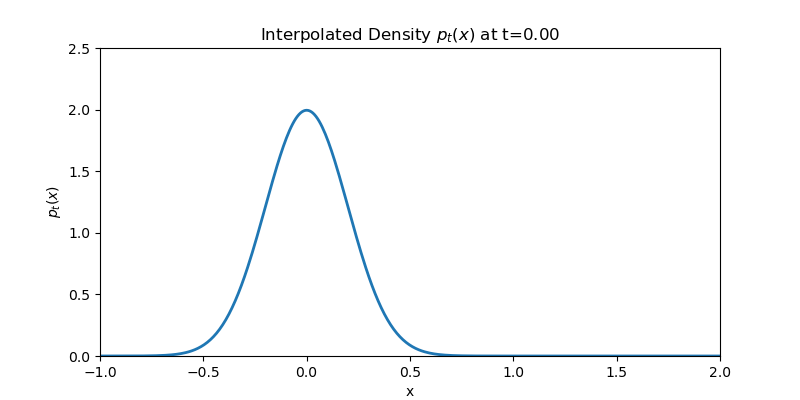
\includegraphics[width=\linewidth]{/home/admin-sbraik/Documents/InternshipProduction/FlowMatching/frames/frame_1.png}
      \caption{}
    \end{subfigure}
    \hfill
    \begin{subfigure}[b]{0.49\textwidth}
      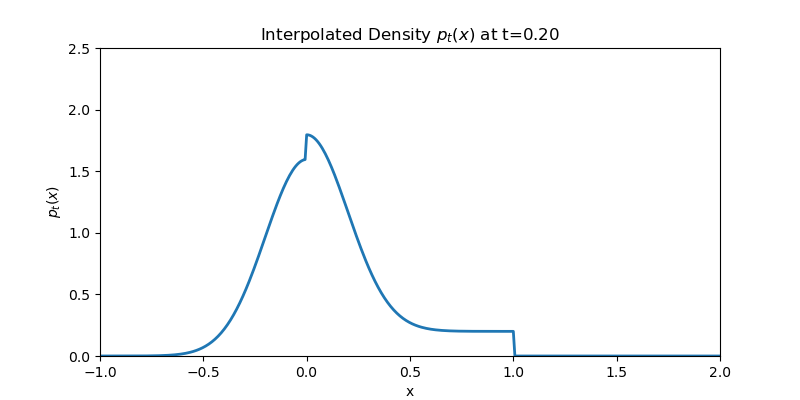
\includegraphics[width=\linewidth]{/home/admin-sbraik/Documents/InternshipProduction/FlowMatching/frames/frame_2.png}
      \caption{}
    \end{subfigure}
    \par\medskip
    \begin{subfigure}[b]{0.49\textwidth}
      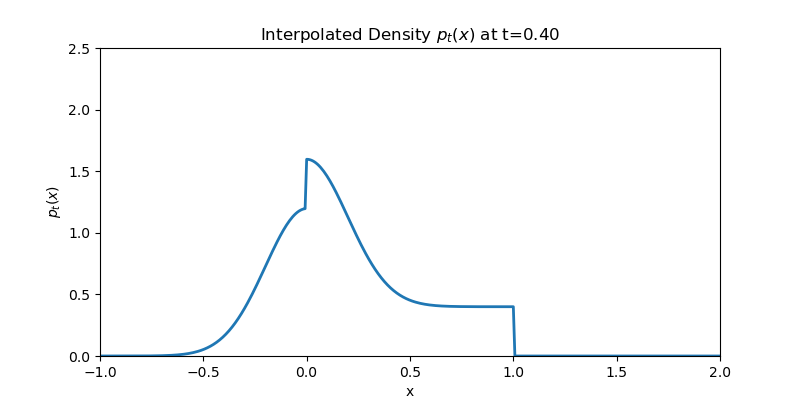
\includegraphics[width=\linewidth]{/home/admin-sbraik/Documents/InternshipProduction/FlowMatching/frames/frame_3.png}
      \caption{}
    \end{subfigure}
    \hfill
    \begin{subfigure}[b]{0.49\textwidth}
      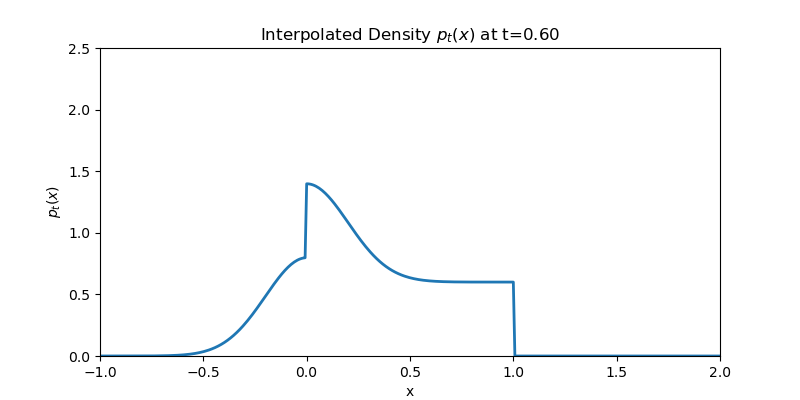
\includegraphics[width=\linewidth]{/home/admin-sbraik/Documents/InternshipProduction/FlowMatching/frames/frame_4.png}
      \caption{}
    \end{subfigure}
    \par\medskip
    \begin{subfigure}[b]{0.49\textwidth}
      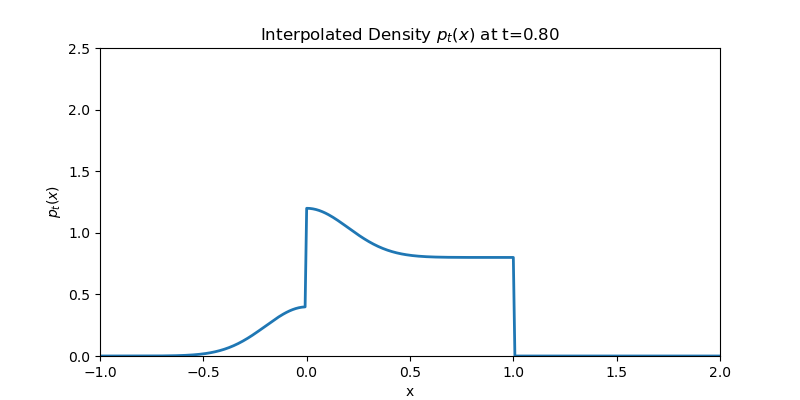
\includegraphics[width=\linewidth]{/home/admin-sbraik/Documents/InternshipProduction/FlowMatching/frames/frame_5.png}
      \caption{}
    \end{subfigure}
    \hfill
    \begin{subfigure}[b]{0.49\textwidth}
      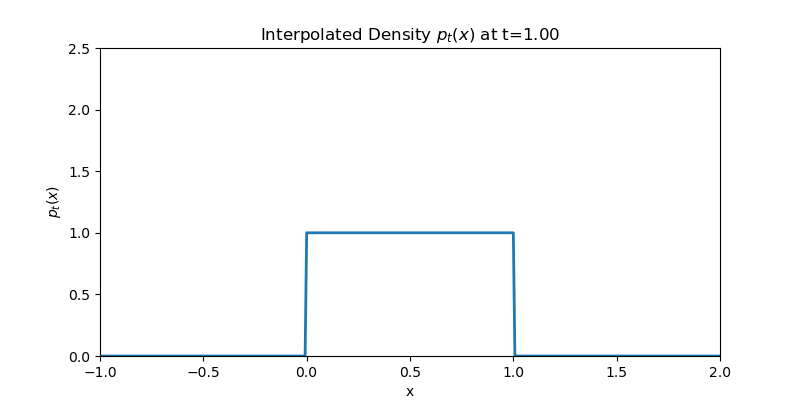
\includegraphics[width=\linewidth]{/home/admin-sbraik/Documents/InternshipProduction/FlowMatching/frames/frame_6.png}
      \caption{}
    \end{subfigure}
    \caption{A probability path interpolating $\mathcal{N}(0,0.2)$ and $\mathcal{U}([0,1])$}
    \label{fig:interpolated_density}
\end{figure}

\newpage

Next we introduce a core object, a time dependant vector field \(v:[0,1]\times \mathbb{R}^d\rightarrow\mathbb{R}^d\) which can be used to construct a map \(\phi:[0,1]\times\mathbb{R}^d\rightarrow\mathbb{R}^d\), called a flow, by the following ODE
\begin{align}
    \frac{d}{dt}\phi_t(x)&=v_t(\phi_t(x))\\
    \quad \phi_0(x)&=x \nonumber
\end{align}  
The link between the flow and the probability path is given by the change of variables formula 
\begin{align}
    p_t(x)=q(\phi_t^{-1}(x))\det \left[\frac{\partial\phi_t^{-1}}{\partial x}(x)\right]
\end{align}
This coincides with the normalizing framework. \\
The link between the vector field and the probability path is given by the continuity equation 
\begin{align}
  \frac{d}{dt}p_t(x)+\text{div}(p_t(x)v_t(x))=0
\end{align}
It said that the vector field \(v_t\) generates the probability path \(p_t\) if the continuity equation holds.\\
\bigskip
\begin{figure}[h]
    \centering
    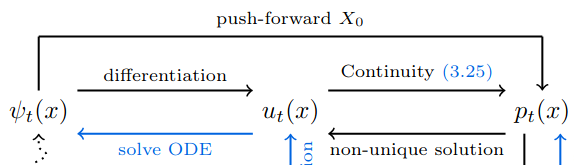
\includegraphics[width=0.8\textwidth]{/home/admin-sbraik/Documents/InternshipProduction/FlowMatching/FlowMatchingBasics.png}
    \caption{How the notions are linked together, from \cite{lipman2024flowmatchingguidecode}}
    \label{fig:flow_matching_basics}
\end{figure}

\subsubsection{Objective}
Given a target probability path \(p_t\) and a corresponding \(v_t\) vector field, the naïve flow matching loss is 

\begin{align}
    \mathcal{L}_\text{FM}(\theta) = \mathbb{E}_{t,p_t(x)}\left[\|v_t^\theta(x)-v_t(x)\|^2\right]
\end{align}

But we don't have acces to \(v_t\) and \(p_t\). To adress this problem and given a particular data sample \(x_1\), we introduce conditional probability path \(p_t(x|x_1)\) such that \(p_0(x|x_1)=q(x)\) at time \(t=0\) and by marginalizing over \(x_1\) we can recover the marginal probability path  
\begin{align}
  p_t(x)=\int p_t(x|x_1)q(x_1)dx_1
\end{align}
So instead of defining a path between two entire distributions, we take a samples from our distributions and we just define how to go from one to the other.\\ 
In the same vein, we can define a conditional vector field, assuming \(p_t(x)\) for all \(t\) and \(x\) 
\begin{align}
  v_t(x)=\int v_t(x|x_1)\frac{p_t(x|x_1)q(x_1)}{p_t(x)}dx_1
\end{align}

\begin{figure}[h]
  \centering
  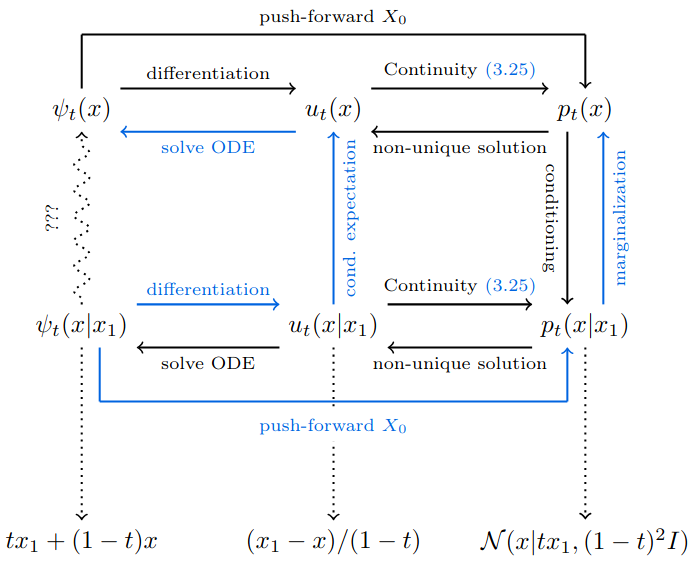
\includegraphics[width=0.8\textwidth]{/home/admin-sbraik/Documents/InternshipProduction/FlowMatching/FlowMatchingFramework.png}
  \caption{A visual in \cite{lipman2024flowmatchingguidecode} that illustates well the full framework}
  \label{fig:flow_matching_framework}
\end{figure}

Then the author introduces a new loss function called the conditional flow matching loss
\begin{align}
  \mathcal{L}_\text{CFM}(\theta) = \mathbb{E}_{t,q(x_1),p_t(x|x_1)}\left[\|v_t^\theta(x|x_1)-v_t(x|x_1)\|^2\right]
\end{align}
with a strong property : \(\mathcal{L}_\text{FM}(\theta)=\mathcal{L}_\text{CFM}(\theta)\) up to a constant independent of \(\theta\). \\
So the focus is now on designing a conditional probability path and vector field and it turns out "the conditional flow matching objective works with any choice of conditional probability path and conditional vector fields". Futhermore, there is an infinite number of vector fields that generate any particular probability path.\\



\subsubsection{Example}
In the original flow matching paper (\cite{lipman2023flowmatchinggenerativemodeling}), they consider the instance of a Gaussian conditional probability path.

\subsection{Diffusion}
The general framework of diffusion is divided in two phases. In the forward phase (noising), we start from a random variable distributed according to our target distribution \( p \), gradually add noise until it reaches an easy-to-sample distribution \(q\) which is practically always a Gaussian. Then, in the backward phase (denoising) we reverse the process and start from \(q\) to get back to \(p\). 

\bigskip

We consider \(T\in\mathbb{N}^{*}\) a finite time horizon, a noise schedule \(\beta:[0,T]\rightarrow \mathbb{R}_{+}^{*}\), assumed to be continuous and non-decreasing, \(B_t\) a Brownian motion at time \(t\).

\textbf{Forward and Backward processes}
\begin{align}
    d\overrightarrow{X}_t = \frac{-\beta(t)}{2\sigma^2}\overrightarrow{X}_t dt + \sqrt{\beta(t)}dB_t, \quad \overrightarrow{X}_0\sim p 
    \quad \text{Forward process}
\end{align} 

\begin{align}
    d\overleftarrow{X}_t=\left(  \frac{\beta(T-t)}{2\sigma^2}\overleftarrow{X}_t+\beta(T-t)\nabla\log p_{T-t}\left(\overleftarrow{X}_t \right)  \right)dt + \sqrt{\beta(T-t)}dB_t, \quad \overleftarrow{X}_0\sim p_T \quad \text{Backward process}
\end{align}

Since we only noise the random variable until a finite time \(T\), the resulting distribution \(p_T\) is not exactly equal to the distribution \(q\), however with a good choice of \(T\) and \(\beta\), we can hope that \(p_T\simeq q\). Furthermore, the backward process allows us to retrieve p but the score \(\nabla p_t\) is unkown at each time \(t\). To adress this problem, denoising score matching is used.  

\bigskip
\textbf{Denoising Score Matching} \newline
Let \(s:\mathbb{R}^d\rightarrow\mathbb{R}^d\). \(X\) a random variable with density \(p\) and \(\varepsilon\) an independant random variable with density \(g\), a centered Gaussian density. Then 

\begin{align}
    \mathbb{E}[|\nabla \log p_t (X+\varepsilon)-s(X+\varepsilon)|^2]&=c+\mathbb{E}[|\nabla \log g(\varepsilon)-s(X+\varepsilon)|^2]\\
    &=c+\mathbb{E}[|(-\varepsilon/\text{Var} (\varepsilon))g(\varepsilon)-s(X+\varepsilon)|^2]
\end{align}
with \(c\) a constant not related to \(s\).

With a good architecural choice of the neural network \(s_\theta\) (data dependent) and noise schedule, we can use the loss to learn the score function and generate new samples from the target distribution using the bakward SDE.

\subsection{Link between flow matching and diffusion}
Diffusion models actually fall in the flow matching framework. Indeed, 

\section{Nonparametric density estimation}
The second approach that could be useful in our situation is nonparametric density estimation. Given an i.i.d. dataset \((X_1,\ldots,X_n)\) drawn from a distribution with density \(f\). The goal, like the name suggests, is to estimate \(f\) without assuming a specific parametric form. The two most common methods are kernel density estimation and projection estimator. 

\subsection{Kernel estimator}
Consider a kernel function \(K\) which is a symmetric density, \(H\) a \(d\times d\) symmetric and positive definite matrix, \(x\in\mathbb{R}^d\), the kernel estimator is defined by 
\begin{align}
\hat{f}_H(x):=\frac{1}{n|\mathrm{H}|^{1/2}}\sum_{j=1}^n K\left(\mathrm{H}^{-1/2}(x-X_j)\right)=\frac{1}{n}K_\mathrm{H}\left(x-X_j\right)
\end{align}
with \(K_\mathrm{H}(x):= |\mathrm{H}|^{-1/2}K(\mathrm{H}^{-1/2}x)\). \\
A widely used kernel is the Gaussian kernel : \(K_\textrm{H}(x)=(2\pi)^{-d/2}|\textrm{H}|^{-1/2}e^{-\frac{1}{2} x^\intercal \textrm{H}^{-1} x}\) \\
The choice of \(\mathrm{H}\) is critical since it governs the bias-variance tradeoff and the convergence rate of the estimator. To choose the optimal \(\mathrm{H}\) few methods could be used like Cross validation or Goldenschlugger-Lepski.

\subsection{Projection estimator}
This method assumes that \(f\in L_2(A), \, A\subset \mathbb{R}^d\). \\
Let \((\varphi_j)_{j\le 1}\) be a Hilbert basis of \(L_2(A)\) such as Fourier, Legendre or wavelets basis. The projection estimator is defined by 

\begin{align}
    \hat{f}_m(x)=\sum_{\|j\|\le m} \hat{a}_j\varphi_j(x), \quad \hat{a}_j=\frac{1}{n}\sum_{i=1}^n \varphi_j(X_i)
\end{align}

\begin{comment}
\begin{align}
    \hat{f}_\mathrm{K}=\sum_{k_1=1}^{K_1}\ldots\sum_{k_d=1}^{K_d}\hat{a}_{k_1,\ldots,k_d}\varphi_{k_1,\ldots,k_d}, \quad \hat{a}_{k_1,\ldots,k_d}=\frac{1}{n}\sum_{i=1}^n \varphi_{k_1,\ldots,k_d}(X_i) = \frac{1}{n}\sum_{i=1}^n \prod_{j=1}^d \varphi_{k_j}(X_i)
\end{align}
\end{comment}
Just like the previous case, the choice of \(m\) is crucial, and methods like cross validation and penalization help choosing the best model.

\bigskip
%One of the drawbacks of those two methods is they work well when the number of observations \(n\) is big.

\newpage
\nocite{Coste_2025}
\nocite{lipman2024flowmatchingguidecode}
\nocite{strasman2025analysisnoiseschedulescorebased}
\nocite{battey2014smoothprojecteddensityestimation}
\nocite{dionblanc2025nonparametricdensityestimation}
\nocite{mathieu2024flow}
\bibliographystyle{plain}
\bibliography{references}
\end{document}
